\documentclass[11pt]{report}
%\documentclass[a4paper, 11pt]{article}
%\usepackage{fullpage}
\usepackage[utf8]{inputenc}
\usepackage[english, ngerman]{babel}
\usepackage[T1]{fontenc}
\usepackage{lmodern}
\usepackage{graphicx}
\usepackage{enumitem}
\usepackage[a4paper, total={6in, 8in}]{geometry}

\usepackage{fancyhdr}
 
\pagestyle{fancy}
\fancyhf{}
\rhead{Share\LaTeX}
\lhead{Guides and tutorials}
\rfoot{Page \thepage}

\title{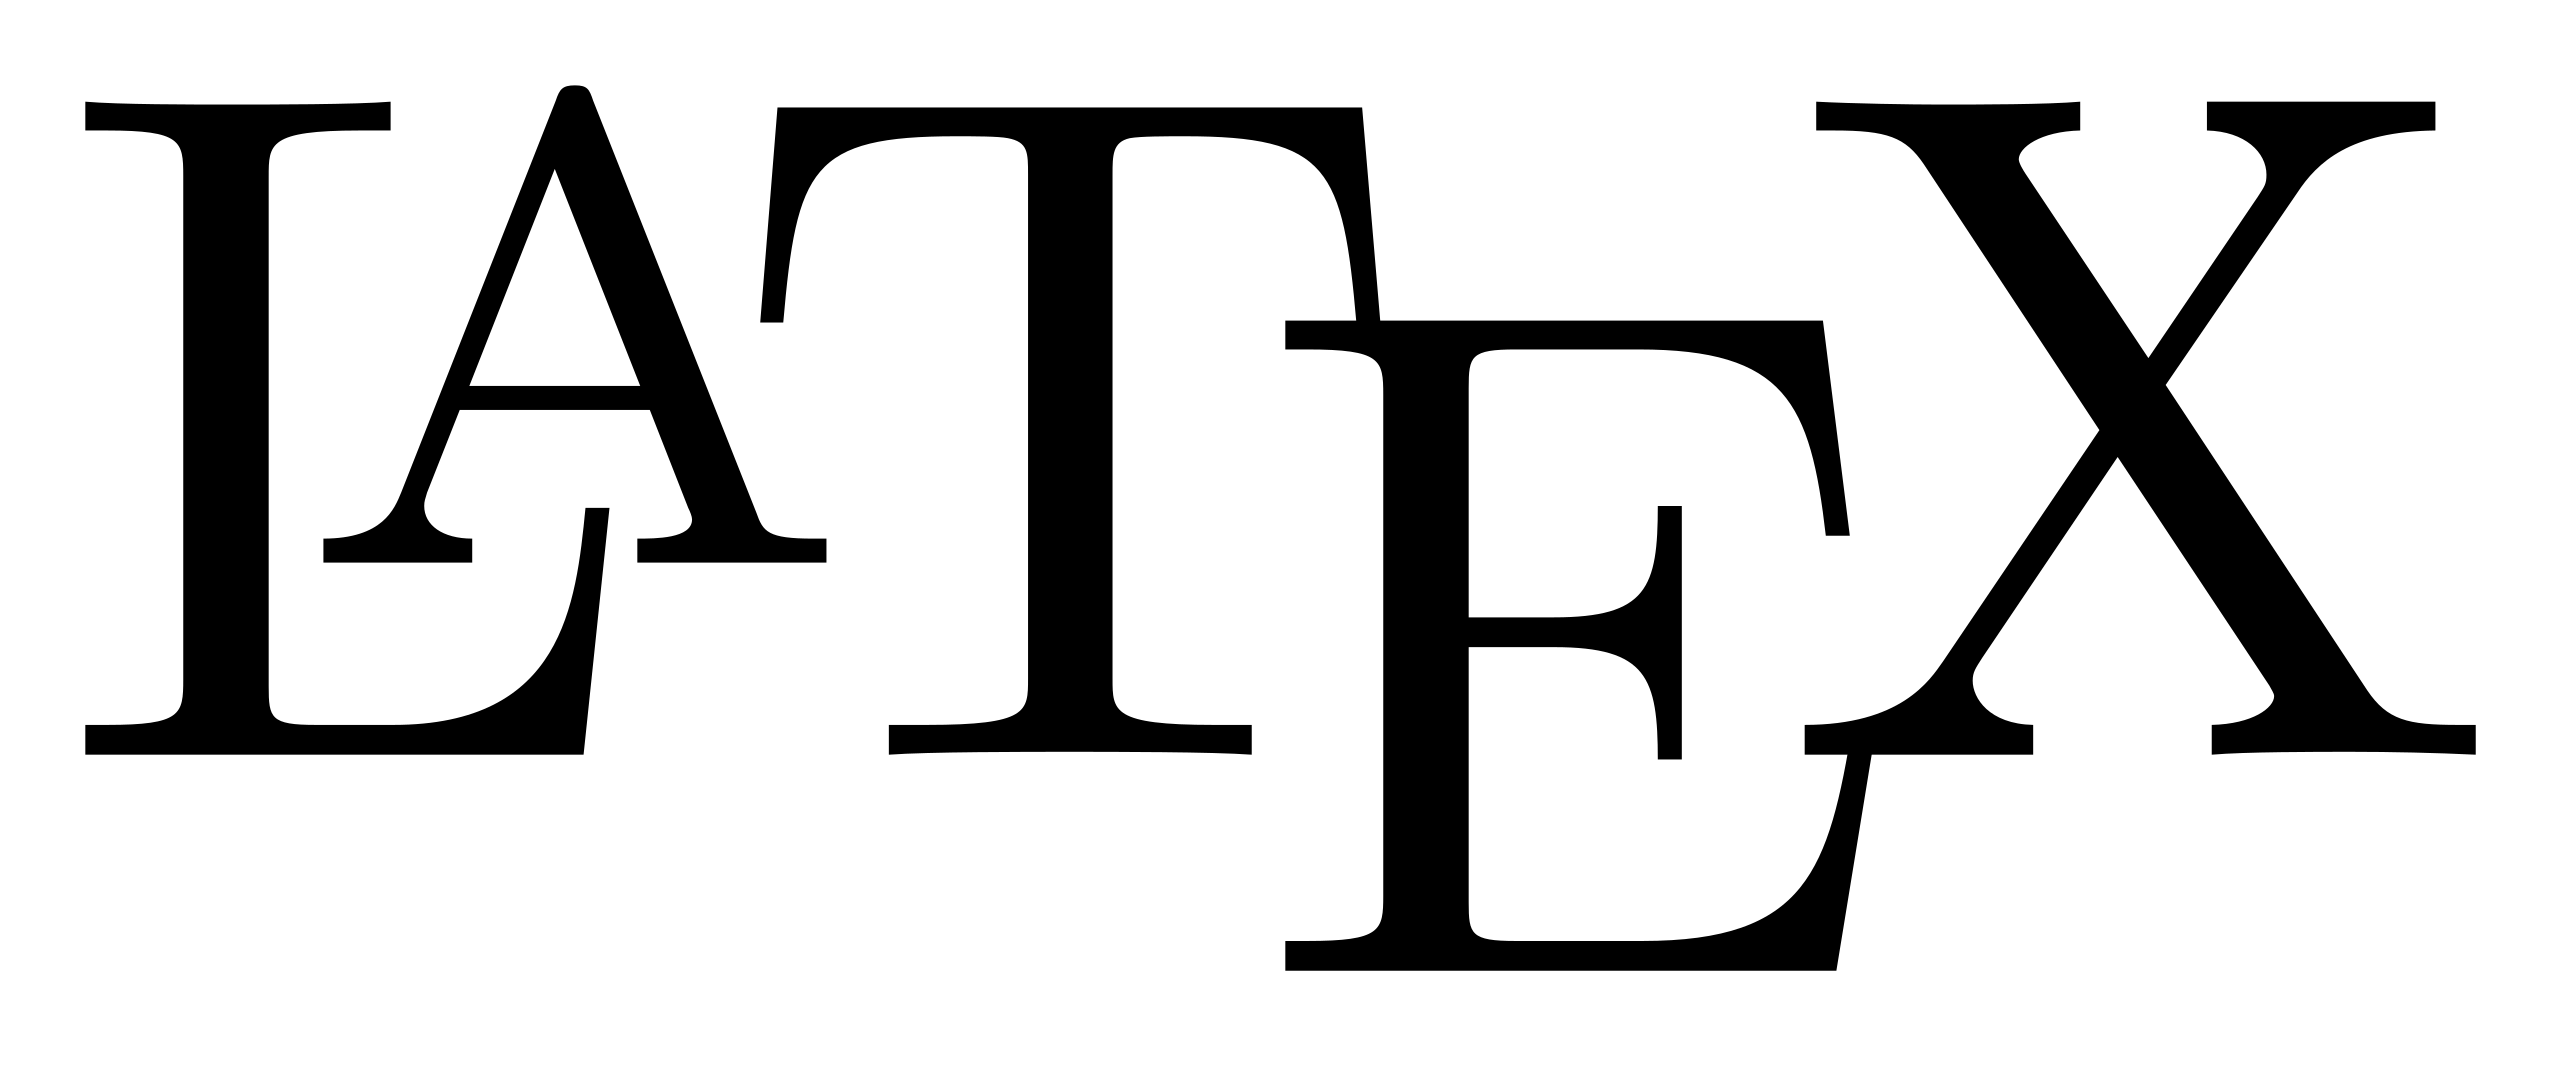
\includegraphics[width=0.5\linewidth]{pics/LaTeXLogo}\\Zusammenfassung}
\author{Silas}
\date{03/14/15}



\begin{document}
\maketitle
\thispagestyle{empty}
Uebersicht ueber diverse Latex-Befehle und wie man diese benutzt.

\textbf{Alle} Befehle \emph{beginnen} mit einem Backslash

\section{Textuelle Darstellung}
\begin{itemize}
  \item \verb|\emph{...}|: hervorgehobener \emph{Text} (Besser als kursiv da Befehl verschachtelt aufgerufen werden kann)
  \item \verb|\textit{...}|: Kursiver \textit{Text}
  \item \verb|\textbf{...}|: Fett gedruckter \textbf{Text}
  \item \verb|\verb|: Quellcode font (quotet alle Latex-Befehle)
  \item \verb|\begin{verbatim*} <Quellcode> \end{verbatim*}|: Darstellung eines gesamten Codeblocks
\end{itemize}

\section{Formatierung}
\begin{itemize}
  \item Listen: 
  \begin{itemize}
  \item geordnet: Beginn mit begin{enumerate}, durchnummerierte Elemente. Elemente mit item ... bezeichnet
  \item ungeordnet: Beginn mit begin{itemize}, Elemente mit item ... angefuehrt
\end{itemize}

\item Ueberschriften
Koennen auch zur Generierung eines Inhaltsverzeichnisses genutzt werden. 
  \item Hauptueberschrift (toplevel): \emph{section}
  \item Unterueberschriften: \emph{subsection}
  \item Unterunterueberschriften: \emph{subsubsection} (tiefer geht es nicht)
  \\Mit dem Zusatz eines Sterns kann die Nummerierung der Ueberschriften vernachlaessigt werden (wird dann aber auch nicht im Inhaltsverzeichnis aufgefuehrt).
  Beispiel: 
  \begin{verbatim*} 
\section{Ueberschrift mit Nummerierung}
\section*{Ueberschrift ohne Nummerierung}
  \end{verbatim*}

  \item \verb|\quad <Text>|: Der Text wird per Tabulator eingerueckt
  \item \verb|\\|: Zeilenumbruch, ansonsten eine neue Leerzeile fuer Paragraphen einfuehren.
\end{itemize}

\subsection{Packages}
Befehl zum einbinden eines Paketes: 
usepackage[<Optionale Parameter>]{<Verpflichtende Parameter}|.
\begin{itemize}
  \item \verb|\usepackage[utf8]{inputenc}|: Deutsche Umlaute werden verfuegbar gemacht emph{(Inputencoding)}
  \item \verb|\usepackage[Tl]{fontenc}|: Kodierung in der PDF-Datei, Umlaute koennen gesucht werden. 
  \item \verb|\usepackage[english, ngerman]{babel}|: Rechtschreibpruefung. Auch mit mehreren Sprach moeglich, letztgenannte immer die Hauptsprache
  \item \verb|\usepackage{lmodern}|: Schoener aussehende Fonts
  \item \verb|\usepackage{graphicx}|: Package zum Einbinden von Bildern
\end{itemize}

\subsection{Klassen}
\begin{itemize}
  \item \verb|documentclass[a4paper]{scrartcl}|: Erneuerte Standarddokumentklasse mit unterschiedlichen Schriften.
\end{itemize}

\subsection{Metadaten}
Erst muessen die Metadaten deklaraiert werden. Dazu einfach die Befehle title, author und date aufrufen. 
\begin{itemize}
  \item \verb|\maketitle|: Muss in einem Dokument aufgerufen werden und erzeugt ein Deckblatt mit den gegebenen Metadaten.
  \item \verb|\thispagestyle{...}|: Der Parameter empty loescht saemtliche Seitenzahlen. 
\end{itemize}

\subsection{Bilder}
Grundsaetlich werden diverse Packages benoetigt um ein Bild einbinden zu koennen. Um nicht jedes mal den Pfad neu eingeben zu muessen gibt es den Befehl \emph{graphicspath}. Ein Aufruf koennte folgendermassen aussehen: 
\begin{itemize}
	\item \verb|\graphicspath{{Bilder/}{foo/}}|: Es koennen so auch mehrere Pfade in einem Aufruf angegeben werden. 
\end{itemize}

\subsection{Sonstiges}
\begin{itemize}[leftmargin=*]
  \item Prozentzeichen zum Auskommentieren 
\end{itemize}

\subsection{Beispielhafter Fliesstext}
asdf asd fas das dfasd fasd fasd fsad fasd fas dfasd asdf asdf asd fas das dfasd fasd fasd fsad fasd fas dfasd asdf asdf asd fas das dfasd fasd fasd fsad fasd fas dfasd asdf asdf asd fas das dfasd fasd fasd fsad fasd fas dfasd asdf asdf asd fas das dfasd fasd fasd fsad fasd fas dfasd asdf asdf asd fas das dfasd fasd fasd fsad fasd fas dfasd asdf asdf asd fas das dfasd fasd fasd fsad fasd fas dfasd asdf asdf asd fas das dfasd fasd fasd fsad fasd fas dfasd asdf asdf asd fas das dfasd fasd fasd fsad fasd fas dfasd asdf 



\end{document}
